\section*{Problem 2}
\begin{itemize}
     \item[A.]{Training VAE}\\
     We used the given architecture and ADAM with the provided learning rate. After training the model for 20 Epochs, we achieved an average value of ELBO of $-93.58$ on validation set. It is clearly higher than the reference value provided in question.  
     
     \item[B.1]{Evaluating log-likelihood with VAE}\\
     Here we implement the Importance Sampling procedure that takes as parameters the trained model, an array of $x_i$ and an array of samples $z_{ik}$ from the distribution $q(z|x_i)$. The procedure returns an array of log-likelihood $\log p(x_i)$  of the size of the mini-batches.The code snippet below demonstrates our implementation. 
     \begin{lstlisting}
     def loss_IS(model, true_x, z):

	#Loop over the elements i of batch
	M = true_x.shape[0]

	#Save logp(x)
	logp_x = np.zeros([M])

	#Get mean and std from encoder
	#2 Vectors of 100
	mu, logvar = model.encode(true_x.to(device))
	std = torch.exp(0.5*logvar)

	K = 200

	#Loop over tha batch
	for i in range(M):
		#z_ik
		samples = z[i,:,:]

		#Compute the reconstructed x's from sampled z's
		x = model.decode(samples.to(device))	

		#Compute the p(x_i|z_ik) of x sampled from z_ik
		#Bernoulli dist = Apply BCE
		#Output an array of losses
		true_xi = true_x[i,:,:].view(-1, 784)
		x = x.view(-1, 784)
	
		p_x = true_xi * torch.log(x) + (1.0-true_xi) * torch.log(1-x)
		p_x = torch.sum(-p_x, dim=1)
		
		##q(z_ik¦x_i) follows a normal dist
		#q_z = mgd(samples, mu, std)
		s = std[i, :].view([std.shape[1]])
		m = mu[i, :].view([std.shape[1]])
		
		q_z = multivariate_normal.pdf(samples.cpu().numpy(),mean=m.cpu().numpy(), cov=np.diag(s.cpu().numpy()**2))

		##p(z_ik) follows a normal dist with mean 0/variance 1
		#(64, 100)	
		#Normally distributed with loc=0 and scale=1
		std_1 = torch.ones(samples.shape[1])
		mu_0 = torch.zeros(samples.shape[1])		

		p_z = multivariate_normal.pdf(samples.cpu().numpy(),mean=mu_0.cpu().numpy(), cov=np.diag(std_1.cpu().numpy()**2))

		#Multiply the probablities
		#marginal_likelihood += (p_x * p_z)/q_z
		#Use logsumexp trick to avoid very small prob
		
		logp_x[i] = np.log((1.0/K) * np.sum(np.exp(np.log(p_x.cpu().numpy()) + np.log(p_z) - np.log(q_z))))

	return logp_x
     \end{lstlisting}
     \item[B.2]
     The evaluation of the training model using the ELBO:
     \begin{itemize}
         \item [a.] Validation: $-93.58$
         \item [b.] Test: $-93.63$
     \end{itemize}
     The evaluation of the training model using the log-likelihood:
     \begin{itemize}
         \item [a.] Validation: $*-93.58$
         \item [b.] Test: $*-43.63$
     \end{itemize}
     Below is a sample of the obtained images generated by the trained model:
\begin{figure}
  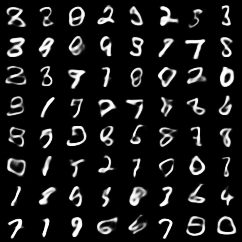
\includegraphics[width=\linewidth]{sample_19.png}
  \caption{A sample of generated images}
  \label{fig:gen_sample}
\end{figure}
\end{itemize}
